% Provenance (never printed): cycle 4 SVT, "La planete Terre": sedimentation,
% from sediment to sedimentary rock, fossilisation, fossils and layers as a
% record of past environments; see sources/book1/PROVENANCE.md. Book 1,
% grade 7, chapter 4.
% Vocabulary guard: first chapter allowed to use "sediment"; the principles of
% relative dating (superposition, fossil succession and the rest) and "unconformity" are
% g7.5's and are not named here; fossils as evidence of evolution are the
% biology books' (one sentence of prose).
\chapter{Sedimen dan Fosil}\label{ch:g7:sediments-and-fossils}

Grand Canyon, di Arizona (Amerika Serikat), dalamnya rata-rata
\qty{1.6}{km}. Dindingnya terdiri atas lapisan-lapisan \omterm{def:g3:stones-pebbles-sand:rock}{batuan}, yang satu di
atas yang lain, berwarna merah, cokelat, kelabu, dan krem. Pada lapisan
paling atas, Batu Kapur Kaibab, para jagawana menunjukkan cangkang-cangkang:
cangkang brakiopoda, hewan yang dulu hidup di dasar \omterm{def:g2:water-on-earth:ocean}{laut}. \omterm{def:g3:stones-pebbles-sand:rock}{Batuan} itu
terbentuk di dasar sebuah \omterm{def:g2:water-on-earth:ocean}{samudra}, dan kini \omterm{def:g3:stones-pebbles-sand:rock}{batuan} itu membentuk bibir
ngarai, tinggi di atas \omterm{def:g4:world-physical-map:altitude}{permukaan laut}.
% ledger: nps:grca-depth, nps:grca-fossils, nps:grca-kaibab

\begin{omfigure}
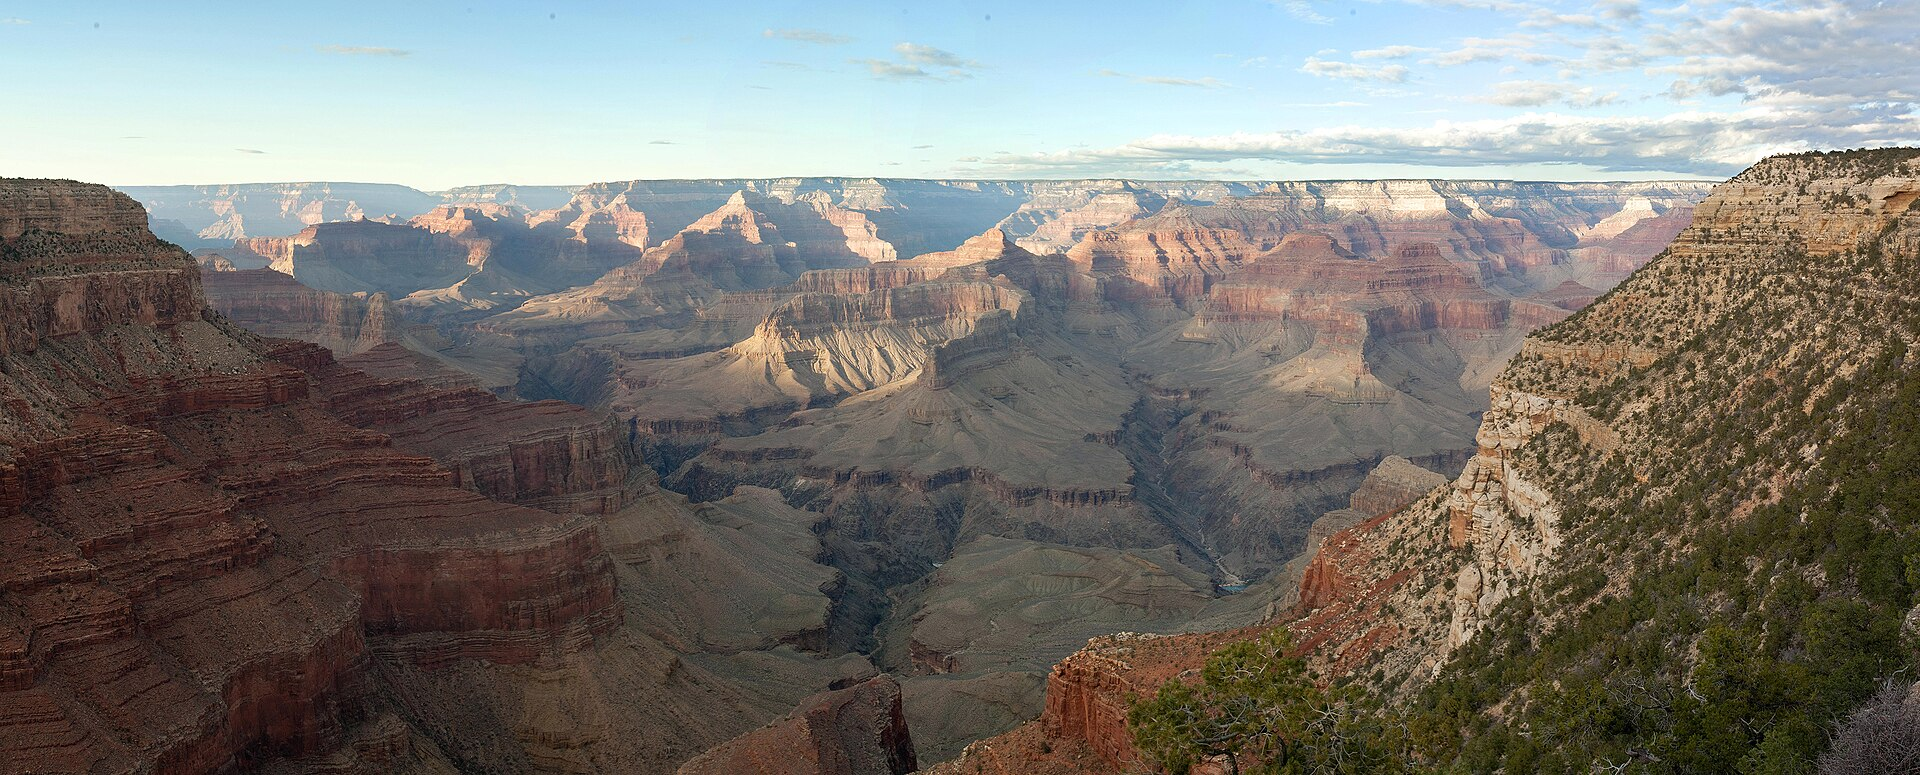
\includegraphics[width=\linewidth]{images/book1/g7-grand-canyon.jpg}

{\small Grand Canyon dilihat dari Hermits Rest, di bibir selatannya: lapis
demi lapis \omterm{def:g3:stones-pebbles-sand:rock}{batuan}, dari bibir ngarai sampai ke dasarnya. Foto NPS karya
Kristen M. Caldon (domain publik, melalui Wikimedia Commons).}
% ledger: commons:grand-canyon
\label{fig:g7:sediments-and-fossils:canyon}
\end{omfigure}

Bagaimana setumpuk \omterm{def:g3:stones-pebbles-sand:sand}{pasir} dan \omterm{def:g3:stones-pebbles-sand:sand}{lumpur} yang lepas menjadi \omterm{def:g3:stones-pebbles-sand:rock}{batuan} yang padat?
Bagaimana sebuah cangkang dapat bertahan begitu lama sehingga akhirnya
berada di dalam tebing? Dan apa yang diceritakan lapisan-lapisan dan \omterm{def:g7:sediments-and-fossils:fossil}{fosil}
kepada kita tentang tempat-tempat seperti keadaannya dahulu kala?

\begin{recall}
Di permukaan, \omterm{def:g3:stones-pebbles-sand:rock}{batuan} perlahan-lahan dipecah menjadi kepingan-kepingan
(\emph{\omterm{def:g5:water-shapes-the-land:weathering}{pelapukan}}); air, angin, dan es membawa kepingan-kepingan itu pergi
(\emph{\omterm{def:g5:water-shapes-the-land:erosion}{erosi}}) dan meletakkannya di tempat kepingan itu melambat dan
berhenti (\emph{\omterm{def:g5:water-shapes-the-land:deposition}{pengendapan}}): yang paling berat lebih dahulu, \omterm{def:g3:stones-pebbles-sand:sand}{lumpur} halus
hanya di tempat airnya hampir diam (\cref{ch:g5:water-shapes-the-land}).
Yang disebut \emph{\omterm{def:g6:rocks-and-minerals:rock-families}{batuan sedimen}} terbentuk di permukaan dari butir-butir
\omterm{def:g3:stones-pebbles-sand:sand}{pasir} dan \omterm{def:g3:stones-pebbles-sand:sand}{lumpur}, atau dari cangkang, yang diendapkan berlapis-lapis lalu
mengeras: batu pasir, serpih, batu kapur. \omterm{def:g6:rocks-and-minerals:rock-cycle}{Siklus batuan} perlahan-lahan
mengubah \omterm{def:g3:stones-pebbles-sand:rock}{batuan} dari setiap keluarga menjadi \omterm{def:g3:stones-pebbles-sand:rock}{batuan} keluarga lain
(\cref{ch:g6:rocks-and-minerals}).
\end{recall}

\section{Sedimen mengendap berlapis-lapis}

Di mana pun air, angin, atau es menjatuhkan apa yang dibawanya, endapan
yang lepas menumpuk: \omterm{def:g3:stones-pebbles-sand:pebble}{kerikil} dan \omterm{def:g3:stones-pebbles-sand:sand}{pasir} di dasar \omterm{def:g1:landscapes-around-us:water}{sungai}, \omterm{def:g3:stones-pebbles-sand:sand}{lumpur} di dasar
\omterm{def:g1:landscapes-around-us:water}{danau}, \omterm{def:g3:stones-pebbles-sand:sand}{pasir} di pantai atau di \omterm{def:g1:landscapes-around-us:landform}{bukit} \omterm{def:g3:stones-pebbles-sand:sand}{pasir}, cangkang di dasar \omterm{def:g2:water-on-earth:ocean}{laut}.

\begin{definition}[Sedimen]\label{def:g7:sediments-and-fossils:sediment}
Yang disebut \emph{sedimen}\index{sedimen} adalah bahan lepas yang
diendapkan oleh air, angin, atau es: \omterm{def:g3:stones-pebbles-sand:pebble}{kerikil}, \omterm{def:g3:stones-pebbles-sand:sand}{pasir}, \omterm{def:g3:stones-pebbles-sand:sand}{lumpur}, atau cangkang
dan kerangka makhluk hidup. Sedimen berkumpul di dasar \omterm{def:g1:landscapes-around-us:water}{sungai}, \omterm{def:g1:landscapes-around-us:water}{danau}, dan
\omterm{def:g2:water-on-earth:ocean}{laut}, dan di darat di tempat angin atau es menjatuhkannya.
\end{definition}

\omterm{def:g7:sediments-and-fossils:sediment}{Sedimen} mengendap dengan urutan tertentu. Ketika air berlumpur melambat,
butir-butir yang paling besar dan paling berat tenggelam lebih dahulu dan
yang paling kecil dan paling ringan paling akhir. Setiap kali keadaan airnya
berubah --- \omterm{def:g5:water-shapes-the-land:flood}{banjir} yang membawa \omterm{def:g3:stones-pebbles-sand:sand}{pasir}, lalu minggu-minggu yang tenang ketika
hanya \omterm{def:g3:stones-pebbles-sand:sand}{lumpur} halus yang mencapai dasar --- butir-butir yang mengendap juga
berubah, dan lapisan baru dimulai. Sedikit demi sedikit, dasar \omterm{def:g1:landscapes-around-us:water}{danau} atau
\omterm{def:g2:water-on-earth:ocean}{laut} tertutup oleh setumpuk lapisan, yang paling tua di bagian bawah
tumpukan.
% ledger: usgs:strata, usgs:sediments-to-rock

\begin{omfigure}
\begin{tikzpicture}[font=\small, x=1cm, y=1cm]
  % land and river
  \fill[omLithAlluv] (0,3.0) -- (2.0,2.45) -- (2.0,0) -- (0,0) -- cycle;
  \fill[blue!35] (0,3.05) -- (2.0,2.5) -- (2.0,2.4) -- (0,2.95) -- cycle;
  % lake water
  \fill[omSea!45] (2.0,2.5) -- (12.4,2.5) -- (12.4,1.12) -- (3.0,1.2) -- cycle;
  \draw[blue!50!black, line width=0.6pt] (2.0,2.5) -- (12.4,2.5);
  % layers on the bottom: thick near the mouth, thinner far out
  \foreach \k/\c in {0/omLithSand, 1/omLithShale, 2/omLithSand, 3/omLithShale} {
    \pgfmathsetmacro{\yb}{0.2+0.25*\k}
    \pgfmathsetmacro{\yt}{0.2+0.25*(\k+1)}
    \fill[\c] (3.0,\yb) -- (12.4,\yb) -- (12.4,\yt-0.08) -- (3.0,\yt) -- cycle;
  }
  \draw[black!60, line width=0.3pt] (3.0,1.2) -- (12.4,1.12);
  \fill[omLithAlluv!80!black] (2.0,0) rectangle (12.4,0.2);
  \fill[omLithAlluv] (2.0,0.2) -- (3.0,0.2) -- (3.0,1.2) -- (2.0,2.45) -- cycle;
  % settling grains: big ones near the mouth, fine ones far out
  \foreach \x/\y in {3.3/2.1, 3.6/1.75, 3.9/2.25, 4.2/1.55, 3.5/1.35, 4.5/2.0} {
    \fill[brown!70!black] (\x,\y) circle (0.07);
    \draw[-{Stealth[length=1.3mm]}, black!60] (\x,\y-0.1) -- (\x,\y-0.32);
  }
  \foreach \x/\y in {6.5/2.2, 7.4/1.8, 8.3/2.15, 9.1/1.6, 9.9/2.05, 10.8/1.75, 11.6/2.1, 7.9/1.35, 10.4/1.3} {
    \fill[brown!50!black] (\x,\y) circle (0.025);
    \draw[-{Stealth[length=1mm]}, black!40] (\x,\y-0.05) -- (\x,\y-0.2);
  }
  \node[anchor=south, align=center] at (1.0,3.1) {sungai yang\\[-2pt]banjir membawa\\[-2pt]pasir dan lumpur};
  \node[anchor=south, align=center] at (4.1,2.55) {pasir mengendap\\[-2pt]lebih dahulu,\\[-2pt]dekat muara};
  \node[anchor=south, align=center] at (9.2,2.55) {lumpur halus mengendap\\[-2pt]perlahan, jauh di tengah,\\[-2pt]tempat airnya tenang};
  \draw[decorate, decoration={brace, amplitude=4pt}] (12.55,1.15) -- (12.55,0.2)
    node[midway, anchor=west, xshift=4pt, align=left, font=\footnotesize] {lapisan di\\[-2pt]dasar: pasir,\\[-2pt]lumpur, pasir,\\[-2pt]lumpur};
\end{tikzpicture}

{\small \omterm{def:g7:sediments-and-fossils:sediment}{Sedimen} yang mengendap di sebuah \omterm{def:g1:landscapes-around-us:water}{danau} (gambar, tidak berskala).
Sesudah setiap \omterm{def:g5:water-shapes-the-land:flood}{banjir}, selapis \omterm{def:g3:stones-pebbles-sand:sand}{pasir} mengendap, lalu \omterm{def:g3:stones-pebbles-sand:sand}{lumpur} halus pada
minggu-minggu tenang sesudahnya: lapis demi lapis menumpuk di dasar.}
% ledger: usgs:strata
\label{fig:g7:sediments-and-fossils:lake}
\end{omfigure}

\begin{definition}[Lapisan sedimen]\label{def:g7:sediments-and-fossils:layer}
Yang disebut \emph{lapisan sedimen}\index{lapisan sedimen}, atau
\emph{stratum}\index{stratum} (jamaknya \emph{strata}), adalah selembar
\omterm{def:g7:sediments-and-fossils:sediment}{sedimen}, atau \omterm{def:g3:stones-pebbles-sand:rock}{batuan} yang terbentuk darinya, yang diendapkan pada satu
waktu. Lapisan itu mempunyai alas dan puncak, dan berbeda dari lapisan di
atas dan di bawahnya dalam ukuran butirnya atau dalam bahan penyusunnya.
\end{definition}

\omterm{def:g7:sediments-and-fossils:sediment}{Sedimen} mengendap dari air atau udara, sehingga \omterm{def:g7:sediments-and-fossils:sediment}{sedimen} diletakkan secara
mendatar, seperti halaman-halaman buku yang tergeletak di atas meja. Jika
lapisan-lapisan ditemukan dalam keadaan miring atau terlipat, ada sesuatu
yang menggerakkannya sesudah lapisan itu terbentuk. Perlapisan adalah tanda
yang paling jelas dari \omterm{def:g6:rocks-and-minerals:rock-families}{batuan sedimen}: kamu sudah melihatnya di dinding
Grand Canyon.
% ledger: usgs:strata, nps:grca-kaibab

\begin{inthelab}[Lapisan di dalam stoples (di kelas, bersama guru)]
Masukkan segenggam \omterm{def:g3:stones-pebbles-sand:pebble}{kerikil}, dua genggam \omterm{def:g3:stones-pebbles-sand:sand}{pasir}, dan beberapa sendok tanah
ke dalam sebuah stoples kaca yang tinggi; isilah dengan air, tutuplah
rapat-rapat, lalu kocoklah. Letakkan stoples itu dan amatilah selama
beberapa menit: \omterm{def:g3:stones-pebbles-sand:pebble}{kerikil} langsung mencapai dasar, \omterm{def:g3:stones-pebbles-sand:sand}{pasir} sedikit kemudian,
dan \omterm{def:g3:stones-pebbles-sand:sand}{lumpur} halus membuat air tetap keruh selama berjam-jam. Keesokan
harinya, tambahkan sedikit tanah dan \omterm{def:g3:stones-pebbles-sand:sand}{pasir} lagi, kocoklah perlahan, dan
biarkan mengendap lagi. Berapa lapisan yang dapat kamu hitung? Butir apa
yang ada di bagian bawah setiap lapisan?
\end{inthelab}

\section{Dari sedimen menjadi batuan}

Sebuah lapisan tidak lama berada di atas. Lapisan-lapisan lain mengendap di
atasnya, lalu yang lain lagi, dan lapisan itu terkubur makin lama makin
dalam. Di bawah berat lapisan-lapisan di atasnya, butir-butirnya tertekan
makin rapat dan air di antaranya terperas keluar. Air yang merembes melalui
tumpukan itu meninggalkan \omterm{def:g6:rocks-and-minerals:mineral}{mineral} di antara butir-butir, semen alami yang
merekatkannya. Dalam waktu yang lama, dengan makin banyaknya lapisan yang
menumpuk dan perubahan kimia yang lambat, \omterm{def:g7:sediments-and-fossils:sediment}{sedimen} lepas di bagian bawah
tumpukan menjadi \omterm{def:g3:stones-pebbles-sand:rock}{batuan}.
% ledger: usgs:sediments-to-rock, usgs:sedimentary

Setiap jenis \omterm{def:g7:sediments-and-fossils:sediment}{sedimen} menghasilkan \omterm{def:g3:stones-pebbles-sand:rock}{batuannya} sendiri.

\begin{center}
\small
\begin{tabular}{|l|l|}
\hline
\textbf{\omterm{def:g7:sediments-and-fossils:sediment}{sedimen}} & \textbf{\omterm{def:g3:stones-pebbles-sand:rock}{batuan} yang terbentuk darinya} \\
\hline
\omterm{def:g3:stones-pebbles-sand:pebble}{kerikil} dan \omterm{def:g3:stones-pebbles-sand:pebble}{kerakal} & konglomerat \\
\omterm{def:g3:stones-pebbles-sand:sand}{pasir} & batu pasir \\
\omterm{def:g3:stones-pebbles-sand:sand}{lumpur} & batu \omterm{def:g3:stones-pebbles-sand:sand}{lumpur}, atau serpih jika terbelah menjadi lembaran tipis \\
cangkang dan kerangka & batu kapur \\
sisa tumbuhan yang terkubur di rawa & batu bara \\
\hline
\end{tabular}
\end{center}
% ledger: usgs:sediments-to-rock, usgs:sedimentary, usgs:coal-origin

\begin{omfigure}
\begin{tikzpicture}[font=\small, x=1cm, y=1cm]
  \pgfmathsetseed{11}
  \foreach \p/\gap/\title in {0/0.40/{sedimen lepas}, 1/0.31/{terkubur dan tertekan:\\[-2pt]air terperas keluar}, 2/0.31/{tersemen: sebuah batuan}} {
    \begin{scope}[xshift=\p*4.6cm]
      \ifnum\p=2 \fill[black!25] (0,0) rectangle (3.4,3.0);
      \else \fill[omSea!45] (0,0) rectangle (3.4,3.0); \fi
      \foreach \i in {0,...,7} {
        \foreach \j in {0,...,6} {
          \pgfmathsetmacro{\gx}{0.25 + \i*\gap*1.05 + 0.05*rand}
          \pgfmathsetmacro{\gy}{0.25 + \j*\gap + 0.05*rand}
          \pgfmathsetmacro{\gr}{0.13 + 0.03*rand}
          \ifdim\gx pt<3.25pt \ifdim\gy pt<2.85pt
            \fill[omLithSand!80!brown, draw=brown!60!black, line width=0.3pt] (\gx,\gy) circle (\gr);
          \fi\fi
        }
      }
      \draw[black!70, line width=0.6pt] (0,0) rectangle (3.4,3.0);
      \node[anchor=north, align=center] at (1.7,-0.1) {\title};
    \end{scope}
  }
  \draw[-{Stealth[length=2.5mm]}, line width=1pt] (3.6,1.5) -- (4.4,1.5);
  \draw[-{Stealth[length=2.5mm]}, line width=1pt] (8.2,1.5) -- (9.0,1.5);
  \foreach \x in {5.3,6.3,7.3} \draw[-{Stealth[length=2mm]}, line width=0.8pt] (\x,3.7) -- (\x,3.1);
  \node[anchor=south] at (6.3,3.7) {berat lapisan-lapisan di atasnya};
  \node[anchor=south, font=\footnotesize, align=center] at (10.9,3.05) {kelabu: semen alami};
\end{tikzpicture}

{\small Dari \omterm{def:g3:stones-pebbles-sand:sand}{pasir} menjadi batu pasir (gambar butir-butirnya, diperbesar
jauh). Kiri: butir-butir lepas dengan air di antaranya. Tengah: terkubur di
bawah lapisan-lapisan baru, butir-butir itu tertekan rapat. Kanan: \omterm{def:g6:rocks-and-minerals:mineral}{mineral}
yang ditinggalkan air merekatkan butir-butir itu.}
% ledger: usgs:sediments-to-rock, usgs:sedimentary
\label{fig:g7:sediments-and-fossils:to-rock}
\end{omfigure}

Sebagian besar \omterm{def:g3:stones-pebbles-sand:rock}{batuan} yang dapat kamu lihat di permukaan Bumi adalah
\omterm{def:g6:rocks-and-minerals:rock-families}{batuan sedimen}. Tumpukan lapisan yang dibentuknya adalah buku sejarah
tempat itu: setiap lapisan adalah satu halaman, dan halaman-halaman yang
paling tua berada di bagian bawah.
% ledger: usgs:sediments-to-rock

\section{Bagaimana fosil terbentuk}

\begin{definition}[Fosil]\label{def:g7:sediments-and-fossils:fossil}
Yang disebut \emph{fosil}\index{fosil} adalah sisa, atau jejak, makhluk
hidup dari masa lampau yang tersimpan di dalam \omterm{def:g3:stones-pebbles-sand:rock}{batuan}. Sebagian fosil
adalah bagian tubuh yang keras --- cangkang, tulang, gigi, kayu --- yang
telah berubah menjadi batu. Fosil yang lain hanya menyimpan bentuk:
\emph{cetakan}\index{cetakan (fosil)} adalah jejak berongga yang tertinggal
di dalam \omterm{def:g3:stones-pebbles-sand:rock}{batuan} di tempat cangkang atau tulang telah larut;
\emph{tuangan}\index{tuangan (fosil)} adalah salinan yang terbentuk ketika
cetakan terisi oleh bahan \omterm{def:g6:rocks-and-minerals:mineral}{mineral} atau \omterm{def:g7:sediments-and-fossils:sediment}{sedimen} baru. Yang disebut
\emph{fosil jejak}\index{fosil jejak} adalah tanda dari apa yang dilakukan
seekor hewan --- jejak kaki, liang, jalur --- dan bukan bagian dari
tubuhnya.
\end{definition}

Sebuah \omterm{def:g7:sediments-and-fossils:fossil}{fosil} memulai hidupnya sebagai hewan atau tumbuhan mati di dasar
\omterm{def:g2:water-on-earth:ocean}{laut} atau \omterm{def:g1:landscapes-around-us:water}{danau}. Jika tetap tidak tertutup, bakteri menguraikannya dan air
perlahan-lahan melarutkan sisanya. \omterm{def:g7:sediments-and-fossils:fossil}{Fosil} hanya punya peluang jika cepat
terkubur, di bawah \omterm{def:g7:sediments-and-fossils:sediment}{sedimen} yang mengendap di atasnya dan menutupnya rapat.
Kemudian, ketika \omterm{def:g7:sediments-and-fossils:sediment}{sedimen} berubah menjadi \omterm{def:g3:stones-pebbles-sand:rock}{batuan}, air yang merembes melalui
lapisan-lapisan membawa \omterm{def:g6:rocks-and-minerals:mineral}{mineral} yang mengisi setiap lubang kecil pada
cangkang atau tulang itu: cangkang atau tulang itu berubah menjadi batu.
Lama sesudahnya, lapisan-lapisan di atasnya dapat terkikis, dan \omterm{def:g7:sediments-and-fossils:fossil}{fosil} itu
muncul di permukaan.
% ledger: ucmp:fossil-conditions, ucmp:fossil-kinds, usgs:sediments-to-rock

\begin{omfigure}
\begin{tikzpicture}[font=\small, x=0.86cm, y=0.86cm,
    shell/.pic={
      \fill[#1] (0,0) circle (0.42);
      \draw[brown!40!black, line width=0.5pt] plot[domain=0:12.5, samples=90, smooth]
        ({0.032*\x*cos(\x r)}, {0.032*\x*sin(\x r)});
      \draw[brown!40!black, line width=0.5pt] (0,0) circle (0.42);
    }]
  % 1: death on the sea floor
  \begin{scope}[xshift=0cm]
    \fill[omSea!45] (0,1.2) rectangle (3.3,3.6);
    \fill[omLithShale] (0,0) rectangle (3.3,1.2);
    \pic at (1.65,1.62) {shell=omLithSand!60!white};
    \node[anchor=north, align=center] at (1.65,-0.1) {1. hewan itu mati\\[-2pt]di dasar laut};
  \end{scope}
  % 2: quick burial
  \begin{scope}[xshift=3.75cm]
    \fill[omSea!45] (0,2.1) rectangle (3.3,3.6);
    \fill[omLithShale] (0,0) rectangle (3.3,1.2);
    \fill[omLithShale!70!white] (0,1.2) rectangle (3.3,2.1);
    \pic at (1.65,1.62) {shell=omLithSand!60!white};
    \foreach \x in {0.5,1.2,2.1,2.8} \fill[brown!50!black] (\x,2.4) circle (0.03);
    \node[anchor=north, align=center] at (1.65,-0.1) {2. lumpur cepat\\[-2pt]menutupinya};
  \end{scope}
  % 3: buried deep, turned to stone
  \begin{scope}[xshift=7.5cm]
    \fill[omLithShale!80!black] (0,0) rectangle (3.3,1.2);
    \fill[omLithShale!85!black] (0,1.2) rectangle (3.3,2.1);
    \fill[omLithSand] (0,2.1) rectangle (3.3,2.9);
    \fill[omLithLime] (0,2.9) rectangle (3.3,3.6);
    \pic at (1.65,1.62) {shell=black!35};
    \node[anchor=north, align=center] at (1.65,-0.1) {3. terkubur dalam,\\[-2pt]menjadi batu};
  \end{scope}
  % 4: uncovered by erosion
  \begin{scope}[xshift=11.25cm]
    \fill[white] (0,0) rectangle (3.3,3.6);
    \fill[omLithShale!80!black] (0,0) -- (3.3,0) -- (3.3,2.6) -- (2.4,2.3) -- (1.8,1.95) -- (1.2,1.7) -- (0,1.5) -- cycle;
    \draw[black!35, line width=0.4pt] (0,1.2) -- (3.3,1.2);
    \draw[black!60, line width=0.4pt] (0,1.5) -- (1.2,1.7) -- (1.8,1.95) -- (2.4,2.3) -- (3.3,2.6);
    \pic at (1.65,1.84) {shell=black!35};
    \node[anchor=north, align=center] at (1.65,-0.1) {4. erosi membawanya\\[-2pt]ke permukaan};
  \end{scope}
  \foreach \p in {0,1,2,3} {
    \begin{scope}[xshift=\p*3.75cm]
      \draw[black!70, line width=0.5pt] (0,0) rectangle (3.3,3.6);
    \end{scope}
  }
\end{tikzpicture}

{\small Bagaimana \omterm{def:g7:sediments-and-fossils:fossil}{fosil} terbentuk (gambar, tidak berskala): sebuah cangkang
cepat terkubur di bawah \omterm{def:g3:stones-pebbles-sand:sand}{lumpur}; terkubur lebih dalam di bawah
lapisan-lapisan baru, cangkang itu berubah menjadi batu; lama sesudahnya,
\omterm{def:g5:water-shapes-the-land:erosion}{erosi} mengikis lapisan-lapisan di atasnya dan \omterm{def:g7:sediments-and-fossils:fossil}{fosil} itu muncul di
permukaan.}
% ledger: ucmp:fossil-conditions, ucmp:fossil-kinds
\label{fig:g7:sediments-and-fossils:steps}
\end{omfigure}

Sebagian besar makhluk hidup sama sekali tidak meninggalkan \omterm{def:g7:sediments-and-fossils:fossil}{fosil}. Tubuh
yang lunak membusuk sebelum sempat terkubur; bahkan cangkang dan tulang
pecah atau larut jika lama tergeletak tanpa tertutup. Tempat terbaik untuk
menjadi \omterm{def:g7:sediments-and-fossils:fossil}{fosil} adalah dasar \omterm{def:g2:water-on-earth:ocean}{laut} atau \omterm{def:g1:landscapes-around-us:water}{danau} yang tenang, tempat \omterm{def:g3:stones-pebbles-sand:sand}{lumpur} halus
mengendap di atas sisa-sisa itu dan melindunginya. Itulah sebabnya \omterm{def:g7:sediments-and-fossils:fossil}{fosil}
yang ditemukan di dalam \omterm{def:g3:stones-pebbles-sand:rock}{batuan} sebagian besar berupa cangkang, serta
cangkang-cangkang kecil dan sisa tumbuhan dan hewan mikroskopis; dinosaurus,
\omterm{def:g7:sediments-and-fossils:fossil}{fosil} yang paling terkenal, hanyalah bagian yang sangat kecil darinya.
% ledger: ucmp:fossil-conditions, usgs:fossil-record-shells

\begin{omfigure}
\begin{minipage}[t]{0.49\linewidth}\centering
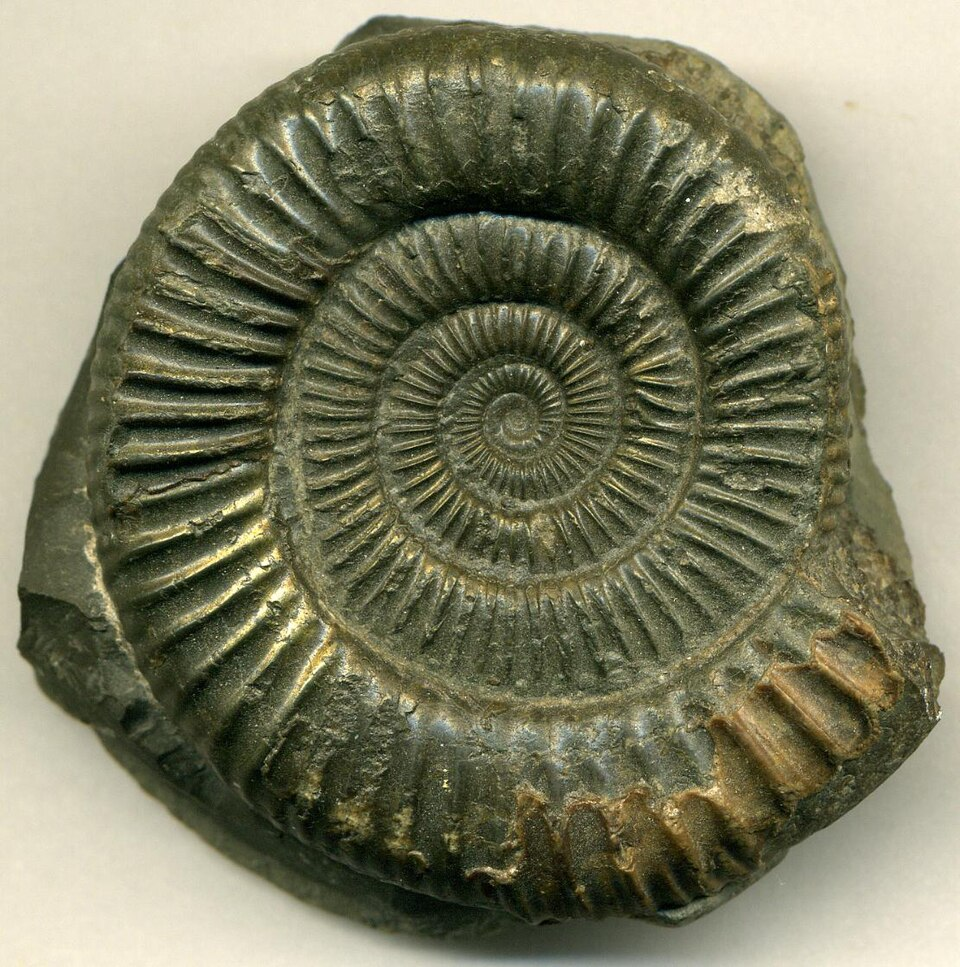
\includegraphics[height=4.6cm]{images/book1/g7-ammonite.jpg}

{\small Sebuah amonit, hewan yang sudah punah dengan cangkang yang
melingkar, kerabat cumi-cumi dan gurita, lebarnya \qty{5.7}{cm}, dari
pantai Yorkshire (Inggris).}
\end{minipage}\hfill
\begin{minipage}[t]{0.49\linewidth}\centering
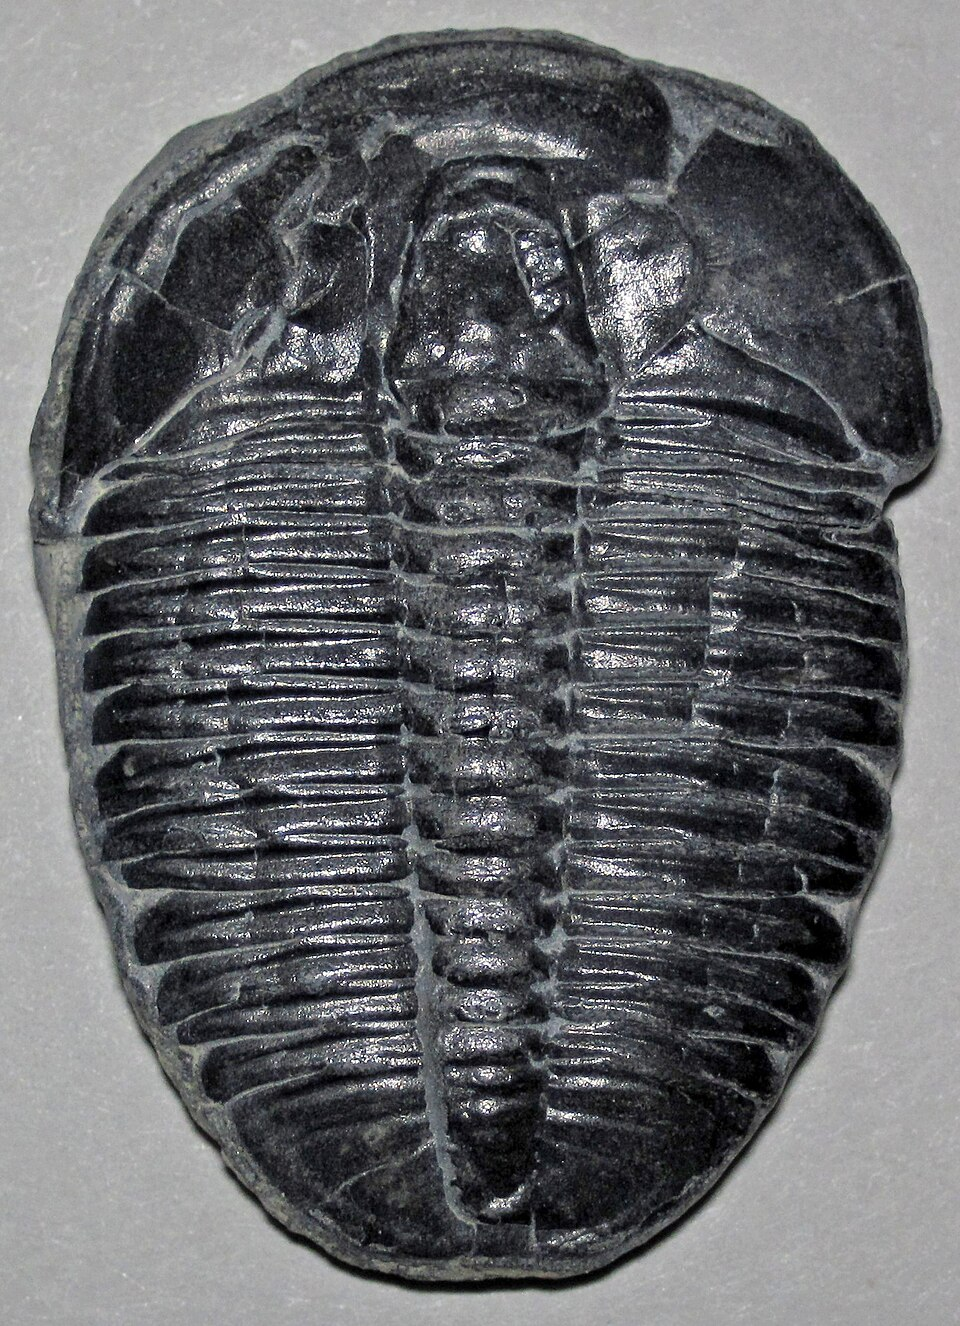
\includegraphics[height=4.6cm]{images/book1/g7-trilobite.jpg}

{\small Sebuah trilobit, hewan \omterm{def:g2:water-on-earth:ocean}{laut} yang sudah punah yang tubuhnya mempunyai
tiga gelambir, lebarnya kira-kira \qty{2.6}{cm}, dari Utah (Amerika Serikat).}
\end{minipage}\par\medskip

{\small Dua \omterm{def:g7:sediments-and-fossils:fossil}{fosil} hewan bercangkang keras. Foto: James
St.~John (CC BY 2.0, melalui Wikimedia Commons).}
% ledger: commons:ammonite, commons:trilobite, nps:ammonoid, nps:trilobite
\label{fig:g7:sediments-and-fossils:ammonite-trilobite}
\end{omfigure}

Kadang-kadang cangkangnya sendiri tidak bertahan. Terkubur di dalam \omterm{def:g3:stones-pebbles-sand:sand}{pasir},
cangkang itu perlahan-lahan dilarutkan oleh air yang merembes di antara
butir-butir, dan hanya tersisa sebuah rongga, dengan bentuk cangkang
tercetak di dindingnya: sebuah \omterm{def:g7:sediments-and-fossils:fossil}{cetakan}. Jika kemudian \omterm{def:g6:rocks-and-minerals:mineral}{mineral} mengendap di
dalam rongga itu dan mengisinya, \omterm{def:g6:rocks-and-minerals:mineral}{mineral} itu membentuk salinan cangkang:
sebuah \omterm{def:g7:sediments-and-fossils:fossil}{tuangan}.
% ledger: ucmp:casts-molds

\begin{omfigure}
\begin{tikzpicture}[font=\small, x=1cm, y=1cm,
    clam/.style={line width=0.5pt}]
  \foreach \p/\fillc/\title in {0/{omLithSand!50!white}/{cangkang terkubur\\[-2pt]di dalam pasir}, 1/{white}/{cangkang sudah larut:\\[-2pt]sebuah cetakan}, 2/{black!40}/{mineral mengisi cetakan:\\[-2pt]sebuah tuangan}} {
    \begin{scope}[xshift=\p*4.9cm]
      \fill[omLithSand] (0,0) rectangle (4.2,2.6);
      \foreach \i in {0,...,40} {
        \pgfmathsetmacro{\gx}{0.1+mod(\i*0.53,4.0)}
        \pgfmathsetmacro{\gy}{0.1+mod(\i*0.37,2.4)}
        \fill[brown!60!black] (\gx,\gy) circle (0.025);
      }
      \fill[\fillc, draw=brown!40!black, clam] (0.9,0.9) arc[start angle=180, end angle=0, x radius=1.2, y radius=0.95] -- cycle;
      \ifnum\p=1
        \foreach \a in {25,45,...,155} \draw[brown!50!black, line width=0.4pt] (2.1,0.9) -- ++(\a:0.93 and 0.75);
      \else
        \foreach \a in {25,45,...,155} \draw[brown!40!black, line width=0.4pt] (2.1,0.9) -- ++(\a:1.05 and 0.85);
      \fi
      \draw[black!70, line width=0.5pt] (0,0) rectangle (4.2,2.6);
      \node[anchor=north, align=center] at (2.1,-0.1) {\title};
    \end{scope}
  }
  \draw[-{Stealth[length=2.5mm]}, line width=1pt] (4.3,1.3) -- (4.8,1.3);
  \draw[-{Stealth[length=2.5mm]}, line width=1pt] (9.2,1.3) -- (9.7,1.3);
\end{tikzpicture}

{\small \omterm{def:g7:sediments-and-fossils:fossil}{Cetakan} dan \omterm{def:g7:sediments-and-fossils:fossil}{tuangan} (gambar, penampang melintang \omterm{def:g3:stones-pebbles-sand:rock}{batuan}). \omterm{def:g7:sediments-and-fossils:fossil}{Cetakan}
adalah rongganya, dengan rusuk-rusuk cangkang tercetak di dindingnya;
\omterm{def:g7:sediments-and-fossils:fossil}{tuangan} adalah salinan cangkang dari batu, yang terbuat dari \omterm{def:g6:rocks-and-minerals:mineral}{mineral} yang
mengisinya.}
% ledger: ucmp:casts-molds
\label{fig:g7:sediments-and-fossils:mould-cast}
\end{omfigure}

Hewan juga meninggalkan \omterm{def:g7:sediments-and-fossils:fossil}{fosil} dari apa yang dilakukannya. Hewan yang
berjalan di atas \omterm{def:g3:stones-pebbles-sand:sand}{lumpur} yang lunak dan basah di tepi \omterm{def:g1:landscapes-around-us:water}{sungai} atau di pantai
meninggalkan jejak kaki. Sebagian besar jejak itu tersapu oleh ombak atau
\omterm{def:g5:water-shapes-the-land:flood}{banjir} berikutnya. Tetapi jika \omterm{def:g3:stones-pebbles-sand:sand}{pasir} menutupinya sebelum jejak itu
terhapus, jejak kaki itu terisi, \omterm{def:g3:stones-pebbles-sand:sand}{pasirnya} kemudian berubah menjadi batu
pasir, dan ketika \omterm{def:g3:stones-pebbles-sand:rock}{batuan} itu terbelah di sepanjang lapisannya, tampaklah
jejak kaki itu dan, di sisi yang lain, \omterm{def:g7:sediments-and-fossils:fossil}{tuangannya}.
% ledger: ucmp:footprints

\begin{omfigure}
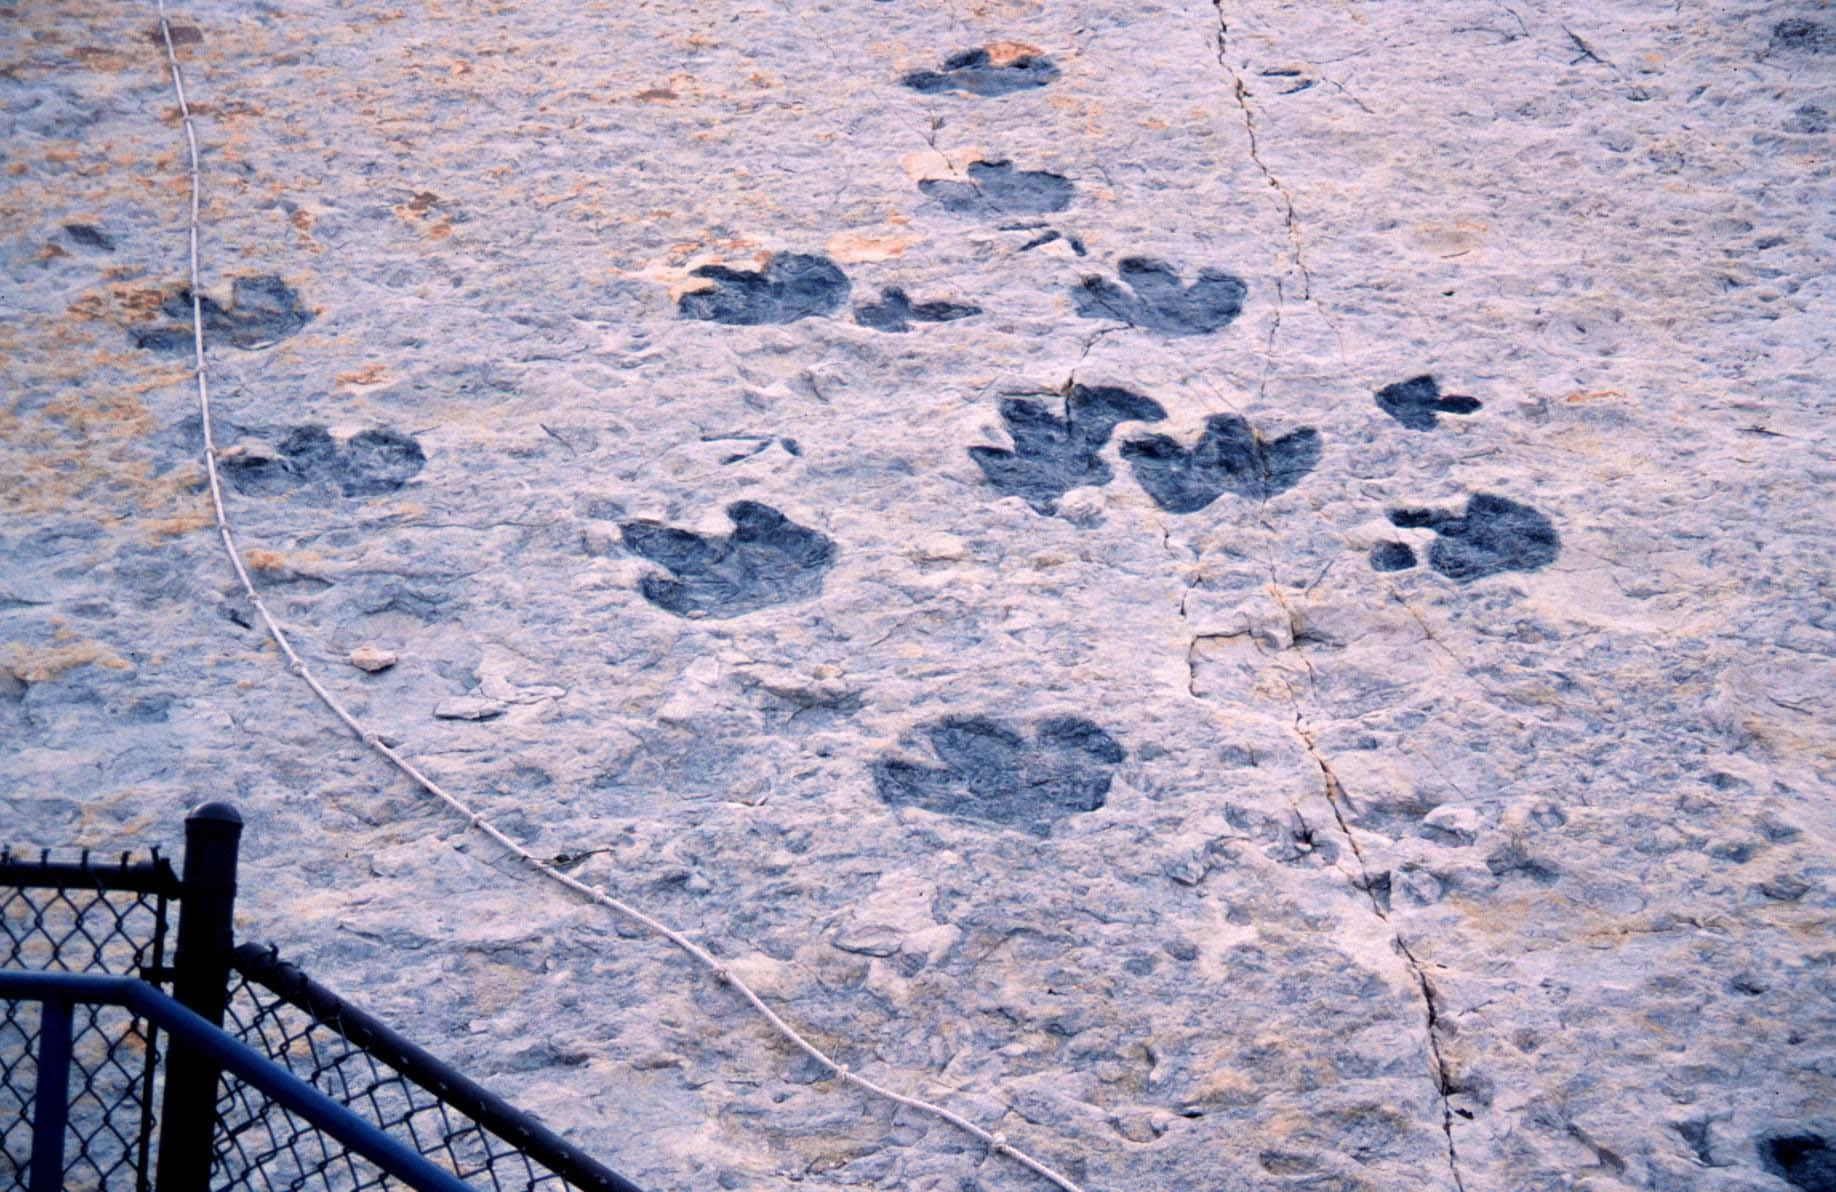
\includegraphics[width=0.62\linewidth]{images/book1/g7-dinosaur-tracks.jpg}

{\small Jejak kaki dinosaurus di Dinosaur Ridge, di dekat Morrison,
Colorado (Amerika Serikat): puluhan jejak yang tertinggal di tanah yang
lunak, kini berupa permukaan \omterm{def:g3:stones-pebbles-sand:rock}{batuan} yang miring. Sebagian besar dibuat
oleh dinosaurus pemakan tumbuhan, beberapa oleh pemakan daging dengan
jari-jari kaki yang ramping. Foto: Dexter Perkins (CC0, melalui Wikimedia
Commons).}
% ledger: commons:dino-tracks
\label{fig:g7:sediments-and-fossils:tracks}
\end{omfigure}

Biologi memakai \omterm{def:g7:sediments-and-fossils:fossil}{fosil} untuk menelusuri sejarah panjang makhluk hidup. Dalam
buku ini, \omterm{def:g7:sediments-and-fossils:fossil}{fosil} adalah petunjuk dari jenis lain: \omterm{def:g7:sediments-and-fossils:fossil}{fosil} memberi tahu kita
seperti apa tempat itu ketika hewan itu hidup di sana.

\section{Lapisan dan fosil, catatan masa lampau}

Setiap lapisan menyimpan tanda-tanda tempat lapisan itu diendapkan. Terumbu
karang kini tumbuh di \omterm{def:g2:water-on-earth:ocean}{laut} yang hangat, jernih, dan dangkal; gelembur
gelombang terbentuk di \omterm{def:g3:stones-pebbles-sand:sand}{pasir} di air yang dangkal, di tepi \omterm{def:g1:landscapes-around-us:water}{danau}, \omterm{def:g1:landscapes-around-us:water}{sungai},
atau \omterm{def:g2:water-on-earth:ocean}{laut}; batu bara terbentuk dari tumbuhan hutan dan rawa purba;
brakiopoda, krinoid, dan trilobit hanya hidup di \omterm{def:g2:water-on-earth:ocean}{laut}. Jika petunjuk yang sama ditemukan pada lapisan yang tua, tempat itu
mungkin seperti itu ketika lapisan itu terbentuk.
% ledger: noaa:coral-where, nps:ripple-marks, nps:ripples-shallow, usgs:coal-origin, nps:trilobite

\begin{center}
\small
\begin{tabular}{|p{0.36\linewidth}|p{0.52\linewidth}|}
\hline
\textbf{petunjuk dalam lapisan} & \textbf{tempat itu ketika lapisan terbentuk} \\
\hline
karang & \omterm{def:g2:water-on-earth:ocean}{laut} yang hangat, dangkal, dan jernih \\
\hline
cangkang hewan \omterm{def:g2:water-on-earth:ocean}{laut} (brakiopoda, krinoid, trilobit) & \omterm{def:g2:water-on-earth:ocean}{laut} \\
\hline
gelembur gelombang di permukaan lapisan & air yang dangkal, di tepi \omterm{def:g1:landscapes-around-us:water}{danau}, \omterm{def:g1:landscapes-around-us:water}{sungai}, atau \omterm{def:g2:water-on-earth:ocean}{laut} \\
\hline
jejak kaki & \omterm{def:g3:stones-pebbles-sand:sand}{lumpur} atau \omterm{def:g3:stones-pebbles-sand:sand}{pasir} yang lunak dan basah, sering di pantai atau di tepi \omterm{def:g1:landscapes-around-us:water}{sungai} \\
\hline
batu bara & hutan rawa atau paya \\
\hline
daun dan sayap capung & daratan yang ditumbuhi tumbuhan \\
\hline
\end{tabular}
\end{center}
% ledger: noaa:coral-where, nps:grca-fossils, nps:trilobite, nps:ripple-marks, nps:ripples-shallow, ucmp:footprints, usgs:coal-origin

\begin{method}[Membaca sebuah lapisan]\label{met:g7:sediments-and-fossils:reading}
\begin{enumerate}
  \item Perhatikan butir-butirnya: butir kasar mengendap di tempat airnya
        bergerak cepat, \omterm{def:g3:stones-pebbles-sand:sand}{lumpur} halus hanya di tempat airnya tenang.
  \item Carilah \omterm{def:g7:sediments-and-fossils:fossil}{fosil} dan tanda-tanda (karang, cangkang, jejak kaki,
        gelembur gelombang, sisa tumbuhan, batu bara) dan gunakan tabel di
        atas.
  \item Gabungkan petunjuk-petunjuk itu menjadi satu gambaran tentang
        tempat itu: darat atau \omterm{def:g2:water-on-earth:ocean}{laut}, dangkal atau dalam, air yang tenang atau
        yang bergerak.
\end{enumerate}
\end{method}

\begin{omfigure}
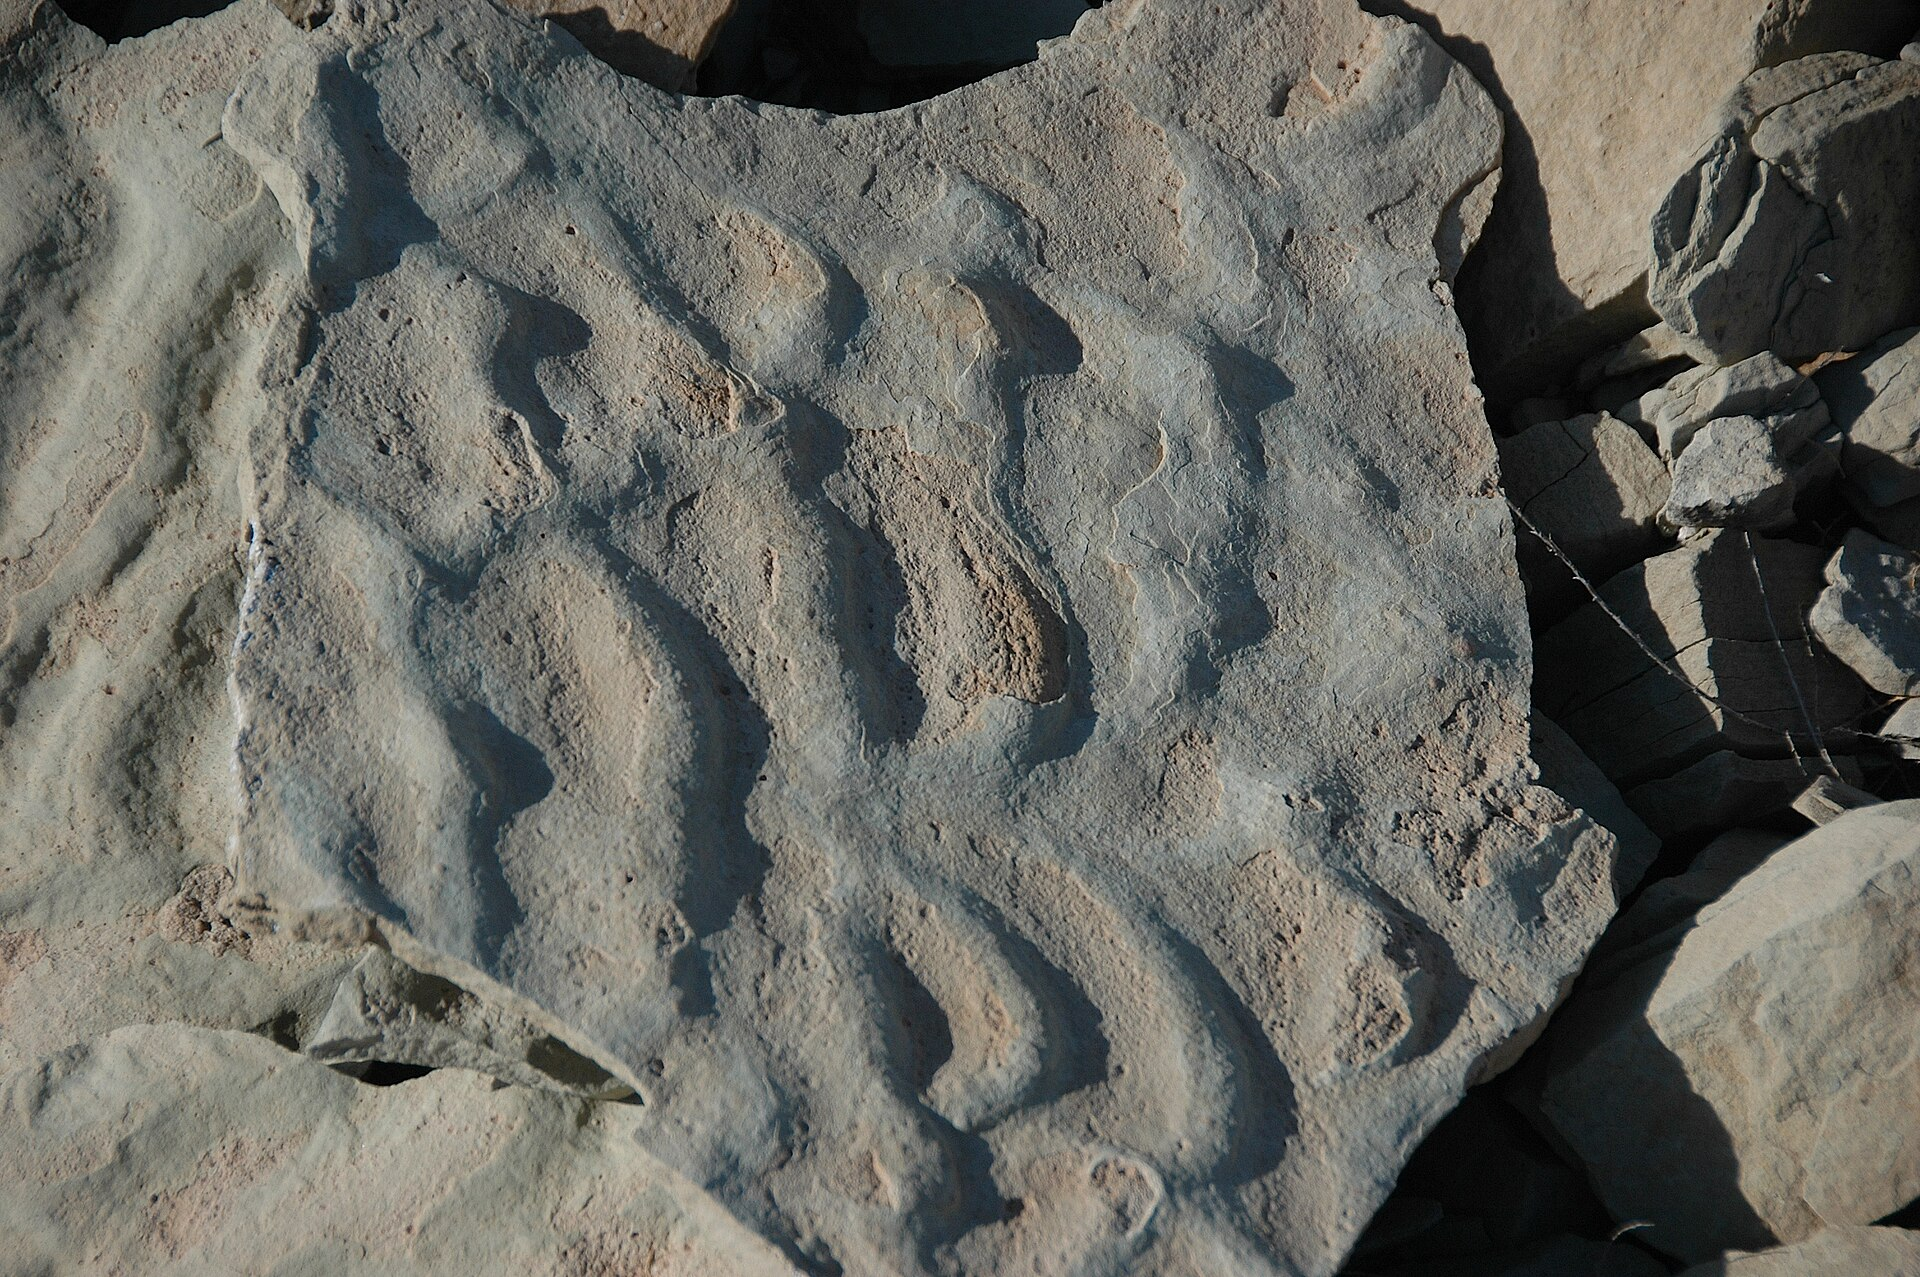
\includegraphics[width=0.56\linewidth]{images/book1/g7-ripple-marks.jpg}

{\small Gelembur gelombang pada sebongkah batu pasir di Taman Nasional
Capitol Reef, Utah (Amerika Serikat): \omterm{def:g3:stones-pebbles-sand:sand}{pasir} itu dulu dibentuk menjadi riak
oleh air yang bergerak, seperti \omterm{def:g3:stones-pebbles-sand:sand}{pasir} di pantai atau di dasar \omterm{def:g1:landscapes-around-us:water}{sungai} kecil
masa kini. Foto: James St.~John (CC BY 2.0, melalui Wikimedia Commons).}
% ledger: commons:ripples, nps:ripple-marks
\label{fig:g7:sediments-and-fossils:ripples}
\end{omfigure}

\begin{example}[Puncak Grand Canyon]\label{ex:g7:sediments-and-fossils:kaibab}
Batu Kapur Kaibab, lapisan teratas Grand Canyon, penuh dengan cangkang
brakiopoda dan potongan batang krinoid, keduanya hewan \omterm{def:g2:water-on-earth:ocean}{laut}. \omterm{def:g3:stones-pebbles-sand:rock}{Batuan} itu
terbentuk di dasar \omterm{def:g2:water-on-earth:ocean}{laut}. Kini lapisan yang sama terletak sampai kira-kira
\qty{2700}{m} (\num{9000}~kaki) di atas \omterm{def:g4:world-physical-map:altitude}{permukaan laut}: sejak lapisan itu
terbentuk, seluruh wilayah itu telah terangkat.
% ledger: nps:grca-fossils, nps:grca-kaibab
\end{example}

Setumpuk lapisan dapat digambar sebagai sebuah \emph{kolom}: lapisan-lapisan
yang disusun menurut urutan terbentuknya, dengan ketebalan yang berskala
dan petunjuk-petunjuknya dicatat di sampingnya. Kolom Perbukitan Varden,
wilayah rekaan untuk latihan-latihan dalam seri ini, ada di bawah ini.

\begin{omfigure}
\begin{tikzpicture}
  \begin{axis}[width=4.2cm, height=9.2cm, scale only axis=false, xmin=0, xmax=1, ymin=-60, ymax=485,
      axis x line=none, axis y line*=left, ytick={0,100,200,300,400},
      ylabel={meter di atas alas batu pasir}, label style={font=\footnotesize},
      tick label style={font=\scriptsize}, clip=false]
    \addplot[lith schist, draw=black!70, line width=0.3pt] table {figdata/out/grade-7-varden_column-unit-older.dat};
    \addplot[lith sandstone, draw=black!70, line width=0.3pt] table {figdata/out/grade-7-varden_column-unit-sandstone.dat};
    \addplot[lith limestone, draw=black!70, line width=0.3pt] table {figdata/out/grade-7-varden_column-unit-limestone.dat};
    \addplot[lith shale, draw=black!70, line width=0.3pt] table {figdata/out/grade-7-varden_column-unit-shale.dat};
    \addplot[om lith={white}{om limestone}, draw=black!70, line width=0.3pt] table {figdata/out/grade-7-varden_column-unit-chalk.dat};
    \node[anchor=west, align=left, font=\footnotesize] at (axis cs:1.12,450) {\textbf{kapur}: puncaknya telah\\terkikis (hanya alasnya yang digambar)};
    \node[anchor=west, align=left, font=\footnotesize] at (axis cs:1.12,350) {\textbf{serpih}, \qty{100}{m}: butir sangat halus;\\amonit};
    \node[anchor=west, align=left, font=\footnotesize] at (axis cs:1.12,210) {\textbf{batu kapur}, \qty{180}{m}:\\karang dan cangkang};
    \node[anchor=west, align=left, font=\footnotesize] at (axis cs:1.12,60) {\textbf{batu pasir}, \qty{120}{m}:\\gelembur gelombang, jejak kaki};
    \node[anchor=west, align=left, font=\footnotesize] at (axis cs:1.12,-30) {batuan yang lebih tua (sekis dan granit),\\terkikis rata sebelum batu pasir datang};
  \end{axis}
\end{tikzpicture}

\medskip
{\small Kolom Perbukitan Varden, wilayah rekaan dalam seri ini:
lapisan-lapisan menurut urutan terbentuknya, yang pertama di bagian bawah,
dengan ketebalan yang berskala. \omterm{def:g7:sediments-and-fossils:fossil}{Fosil} dan tanda yang dicatat di sampingnya
adalah data latihan.}
% ledger: (invented region: figdata/shared/region.py, drawn by figdata/grade-7/varden_column.py)
\label{fig:g7:sediments-and-fossils:column}
\end{omfigure}

\begin{omfigure}
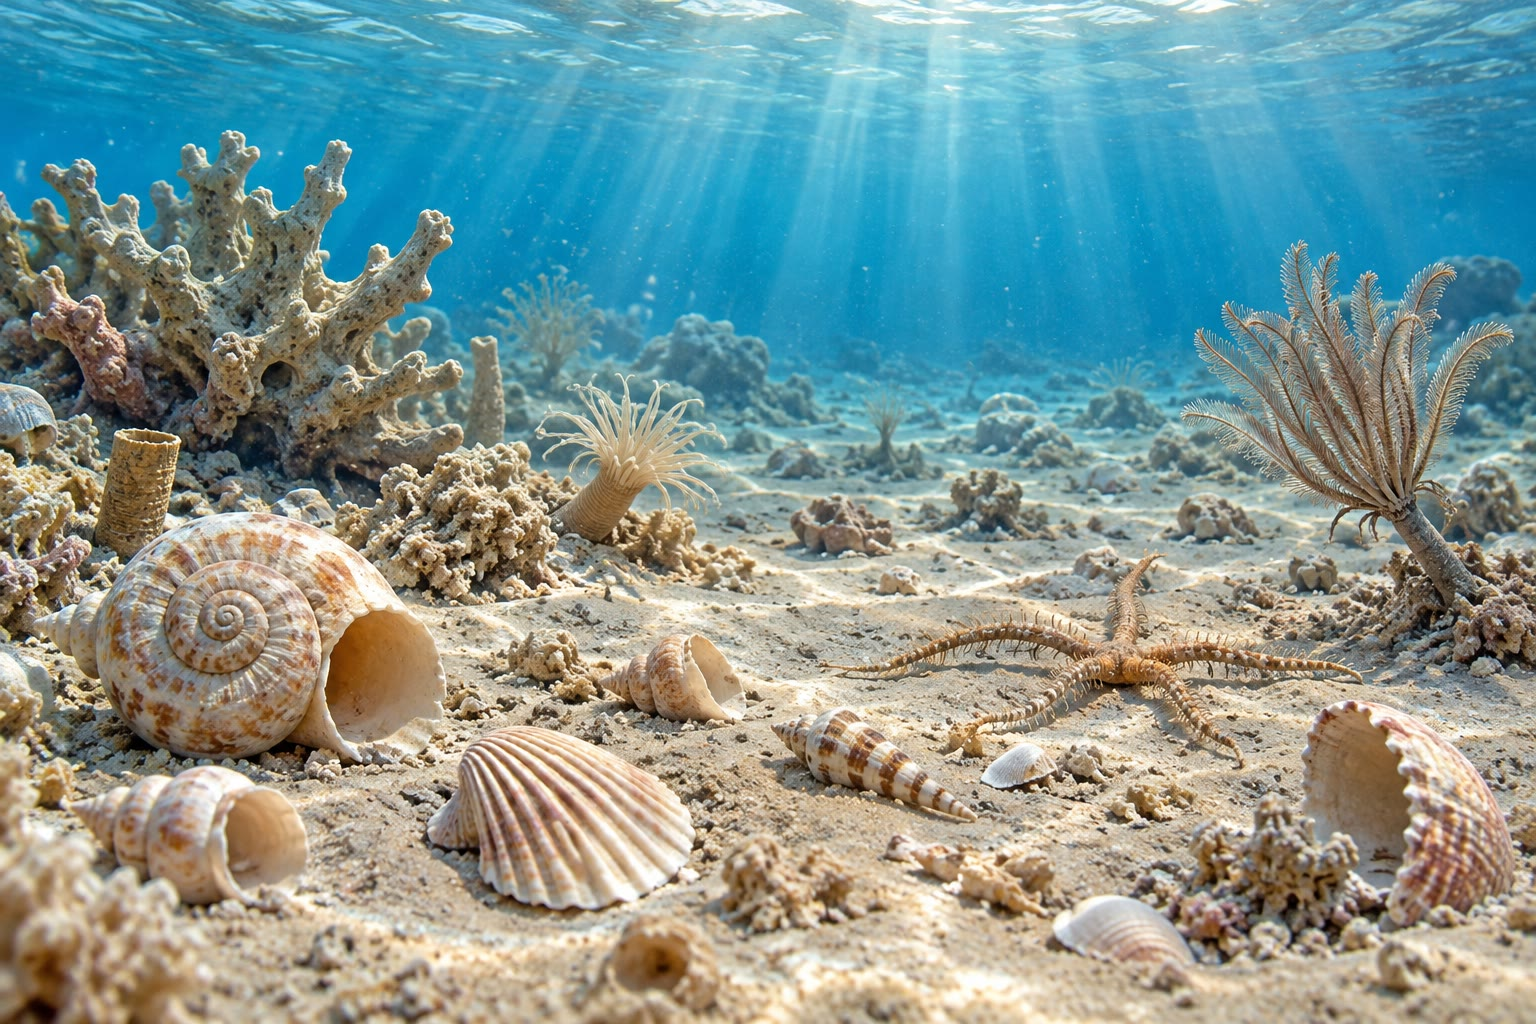
\includegraphics[width=0.6\linewidth]{images/book1/ai/g7-shallow-sea.jpg}

{\small Dasar \omterm{def:g2:water-on-earth:ocean}{laut} yang hangat dan dangkal pada masa lampau, sebagaimana
mungkin tampaknya ketika cangkang dan kepingan karang mengendap menjadi
calon batu kapur (ilustrasi AI dari suatu adegan umum).}
\label{fig:g7:sediments-and-fossils:shallow-sea}
\end{omfigure}

\begin{remark}[Lihat, foto, tinggalkan]\label{rem:g7:sediments-and-fossils:leave}
Di banyak tempat yang dilindungi, mengambil \omterm{def:g7:sediments-and-fossils:fossil}{fosil} dilarang: di Grand
Canyon, misalnya, menggali, memindahkan, atau mengambil \omterm{def:g7:sediments-and-fossils:fossil}{fosil} apa pun
melanggar hukum. Pengunjung yang menemukan \omterm{def:g7:sediments-and-fossils:fossil}{fosil} memotretnya atau
menggambarnya, meninggalkannya di tempatnya agar dapat dilihat orang lain
dan diteliti para ilmuwan, lalu memberi tahu jagawana.
\end{remark}
% ledger: nps:grca-fossils

\begin{inthefield}[Sedimen yang sedang diendapkan pada masa kini]
Di pantai, di tepi \omterm{def:g1:landscapes-around-us:water}{danau}, atau di tepi \omterm{def:g1:landscapes-around-us:water}{sungai} kecil, bersama orang dewasa,
amatilah \omterm{def:g3:stones-pebbles-sand:sand}{pasir} di bawah air yang dangkal: air yang bergerak membentuknya
menjadi riak, seperti riak yang tersimpan di dalam batu pasir yang tua.
Buatlah jejak kaki di \omterm{def:g3:stones-pebbles-sand:sand}{pasir} basah di dekat batas air dan amatilah apa yang
dilakukan ombak-ombak berikutnya terhadapnya. Sesudah hari \omterm{def:g4:clouds-rain-snow:precipitation}{hujan},
amatilah genangan yang sudah kering: selapis tipis \omterm{def:g3:stones-pebbles-sand:sand}{lumpur} halus sering
menutupi \omterm{def:g3:stones-pebbles-sand:sand}{pasir} di dasarnya --- butir-butir yang paling halus mengendap
paling akhir, ketika airnya diam. Gambarlah apa yang kamu lihat, dan
catatlah tempat dan waktunya.
\end{inthefield}
% ledger: nps:ripple-marks, ucmp:footprints, usgs:strata

\section{Latihan}

\begin{exercise}[$\star$]\label{exo:g7:sediments-and-fossils:1}
Pasangkan setiap kata dengan artinya: \omterm{def:g7:sediments-and-fossils:sediment}{sedimen}; \omterm{def:g7:sediments-and-fossils:layer}{stratum}; \omterm{def:g7:sediments-and-fossils:fossil}{fosil}; \omterm{def:g7:sediments-and-fossils:fossil}{cetakan};
\omterm{def:g7:sediments-and-fossils:fossil}{tuangan}; \omterm{def:g7:sediments-and-fossils:fossil}{fosil jejak}. (a) Rongga yang tertinggal di dalam \omterm{def:g3:stones-pebbles-sand:rock}{batuan} di tempat
sebuah cangkang telah larut. (b) Jejak kaki atau liang yang tersimpan di
dalam \omterm{def:g3:stones-pebbles-sand:rock}{batuan}. (c) Bahan lepas yang diendapkan oleh air, angin, atau es.
(d) Salinan dari batu yang terbentuk ketika sebuah rongga terisi \omterm{def:g6:rocks-and-minerals:mineral}{mineral}.
(e) Selembar \omterm{def:g7:sediments-and-fossils:sediment}{sedimen} yang diendapkan pada satu waktu. (f) Sisa atau jejak
makhluk hidup dari masa lampau, yang tersimpan di dalam \omterm{def:g3:stones-pebbles-sand:rock}{batuan}.
\end{exercise}

\begin{exercise}[$\star$]\label{exo:g7:sediments-and-fossils:2}
Urutkan langkah-langkah berikut, untuk menceritakan bagaimana sebuah
cangkang menjadi \omterm{def:g7:sediments-and-fossils:fossil}{fosil} di permukaan: (a) \omterm{def:g5:water-shapes-the-land:erosion}{erosi} mengikis lapisan-lapisan di
atasnya; (b) hewan itu mati di dasar \omterm{def:g2:water-on-earth:ocean}{laut}; (c) lapisan-lapisan baru
menumpuk dan cangkang itu berubah menjadi batu; (d) \omterm{def:g3:stones-pebbles-sand:sand}{lumpur} cepat menutupi
cangkang itu.
\end{exercise}

\begin{exercise}[$\star$]\label{exo:g7:sediments-and-fossils:3}
Gunakan tabel petunjuk. Di mana setiap lapisan terbentuk? (a) Batu kapur
yang penuh karang. (b) Batu pasir yang permukaannya menunjukkan gelembur
gelombang. (c) Lapisan batu bara yang gelap. (d) Serpih dengan \omterm{def:g7:sediments-and-fossils:fossil}{cetakan} daun
dan sayap seekor capung.
\end{exercise}

\begin{exercise}[$\star$]\label{exo:g7:sediments-and-fossils:4}
Benar atau salah? Perbaikilah pernyataan yang salah. (a) Setiap hewan yang
mati suatu hari menjadi \omterm{def:g7:sediments-and-fossils:fossil}{fosil}. (b) Jejak kaki dapat menjadi \omterm{def:g7:sediments-and-fossils:fossil}{fosil}.
(c) Ketika air berlumpur melambat, \omterm{def:g3:stones-pebbles-sand:sand}{lumpur} halus mengendap lebih dahulu.
(d) \omterm{def:g7:sediments-and-fossils:sediment}{Sedimen} diendapkan secara mendatar.
\end{exercise}

\begin{exercise}[$\star\star$]\label{exo:g7:sediments-and-fossils:5}
Gunakan kolom Perbukitan Varden. (a) Sebutkan ketebalan batu pasir, batu
kapur, dan serpih. (b) Berapa ketebalan totalnya? (c) Berapa persen dari
total ini yang berupa batu kapur? Bulatkan ke bilangan bulat terdekat.
(d) Mengapa kolom itu tidak memberikan ketebalan untuk kapur?
\end{exercise}

\begin{exercise}[$\star\star$]\label{exo:g7:sediments-and-fossils:6}
Seorang murid mengocok sebuah stoples berisi air dengan \omterm{def:g3:stones-pebbles-sand:pebble}{kerikil}, \omterm{def:g3:stones-pebbles-sand:sand}{pasir}, dan
\omterm{def:g3:stones-pebbles-sand:sand}{lumpur}, lalu membiarkannya mengendap. (a) Gambarlah stoples itu keesokan
harinya, dan berilah nama pada lapisan-lapisannya. (b) Mengapa airnya masih
keruh sesudah satu jam? (c) Ia menambahkan \omterm{def:g3:stones-pebbles-sand:sand}{pasir} dan \omterm{def:g3:stones-pebbles-sand:sand}{lumpur} lagi lalu
membiarkannya mengendap. Apa yang dilihatnya di dasar sekarang? (d) Lapisan
mana di dalam stoples itu yang terbentuk paling dahulu?
\end{exercise}

\begin{exercise}[$\star\star$]\label{exo:g7:sediments-and-fossils:7}
Manakah di antara benda-benda ini yang paling berpeluang menjadi \omterm{def:g7:sediments-and-fossils:fossil}{fosil}, dan
mana yang paling kecil peluangnya? Jelaskan. (a) Ubur-ubur yang terdampar
di pantai berbatu. (b) Cangkang siput yang terkubur di \omterm{def:g3:stones-pebbles-sand:sand}{lumpur} \omterm{def:g1:landscapes-around-us:water}{danau} yang
tenang. (c) Tulang yang tergeletak bertahun-tahun di \omterm{def:g1:landscapes-around-us:landform}{dataran} yang kering.
(d) Cangkang kerang yang tertutup \omterm{def:g3:stones-pebbles-sand:sand}{pasir} ketika \omterm{def:g1:landscapes-around-us:water}{sungai} \omterm{def:g5:water-shapes-the-land:flood}{banjir}.
\end{exercise}

\begin{exercise}[$\star\star$]\label{exo:g7:sediments-and-fossils:8}
Sebuah cangkang terkubur di dalam \omterm{def:g3:stones-pebbles-sand:sand}{pasir} yang kemudian menjadi batu pasir.
Air yang merembes melalui \omterm{def:g3:stones-pebbles-sand:rock}{batuan} itu melarutkan cangkang itu seluruhnya.
(a) Apa yang tertinggal di dalam \omterm{def:g3:stones-pebbles-sand:rock}{batuan}? (b) Kemudian, \omterm{def:g6:rocks-and-minerals:mineral}{mineral} mengisi
rongga ini. Apa yang terbentuk? (c) Apakah cangkang itu sendiri masih ada?
(d) Mengapa \omterm{def:g7:sediments-and-fossils:fossil}{cetakan} dan \omterm{def:g7:sediments-and-fossils:fossil}{tuangan} lebih sering ditemukan di dalam batu pasir
daripada di dalam serpih? (Pikirkan betapa mudahnya air lewat di antara
butir-butirnya.)
\end{exercise}

\begin{exercise}[$\star\star$]\label{exo:g7:sediments-and-fossils:9}
Grand Canyon dalamnya rata-rata \qty{1.6}{km}. (a) Tuliskan kedalaman ini
dalam meter. (b) Andaikan dinding ngarai itu terdiri atas lapisan-lapisan
yang masing-masing tebalnya \qty{80}{m}: berapa lapisan yang muat dari
bibir sampai ke dasar? (c) Lapisan setebal \qty{160}{m} berapa persen dari
kedalaman itu?
\end{exercise}

\begin{exercise}[$\star\star$]\label{exo:g7:sediments-and-fossils:10}
Jejak kaki dinosaurus ditemukan di dalam batu pasir. (a) Apakah dinosaurus
itu berjalan di atas \omterm{def:g3:stones-pebbles-sand:rock}{batuan} yang keras? Jelaskan. (b) Mengapa sebagian
besar jejak kaki yang ditinggalkan di pantai berlumpur menghilang? (c) Apa
yang harus terjadi tidak lama sesudah dinosaurus itu lewat agar jejak
kakinya tersimpan? (d) Apakah jejak kaki itu \omterm{def:g7:sediments-and-fossils:fossil}{fosil} tubuh atau \omterm{def:g7:sediments-and-fossils:fossil}{fosil jejak}?
\end{exercise}

\begin{exercise}[$\star\star\star$]\label{exo:g7:sediments-and-fossils:11}
Di sebuah \omterm{def:g1:landscapes-around-us:water}{danau}, setiap \omterm{def:g5:water-shapes-the-land:flood}{banjir} meninggalkan selapis \omterm{def:g3:stones-pebbles-sand:sand}{pasir} setebal kira-kira
\qty{2}{cm}, dan minggu-minggu tenang sesudahnya selapis \omterm{def:g3:stones-pebbles-sand:sand}{lumpur} setebal
kira-kira \qty{5}{mm} (data latihan). (a) Berapa tebal, dalam milimeter,
sepasang lapisan? (b) Sebuah \omterm{def:g6:inside-the-earth:layers}{inti} bor yang diambil dari dasar \omterm{def:g1:landscapes-around-us:water}{danau}
panjangnya \qty{1}{m} dan hanya terdiri atas pasangan-pasangan lapisan
seperti itu. Berapa \omterm{def:g5:water-shapes-the-land:flood}{banjir} yang dicatatnya? (c) Di dekat muara \omterm{def:g1:landscapes-around-us:water}{sungai},
lapisan \omterm{def:g3:stones-pebbles-sand:sand}{pasirnya} lebih tebal; jauh di tengah, lebih tipis. Jelaskan
mengapa. (d) Mengapa jauh dari muara ada lebih banyak \omterm{def:g3:stones-pebbles-sand:sand}{lumpur} daripada
\omterm{def:g3:stones-pebbles-sand:sand}{pasir}?
\end{exercise}

\begin{exercise}[$\star\star\star$]\label{exo:g7:sediments-and-fossils:12}
\omterm{def:g7:sediments-and-fossils:fossil}{Fosil} yang ditemukan di dalam \omterm{def:g3:stones-pebbles-sand:rock}{batuan} sebagian besar berupa cangkang dan
sisa-sisa yang kecil; \omterm{def:g7:sediments-and-fossils:fossil}{fosil} hewan bertubuh lunak jarang, dan dinosaurus
hanyalah bagian yang sangat kecil dari semua \omterm{def:g7:sediments-and-fossils:fossil}{fosil}. (a) Jelaskan mengapa
cangkang begitu banyak. (b) Jelaskan mengapa hewan bertubuh lunak jarang.
(c) Seorang ilmuwan ingin mengetahui semua hewan yang hidup di sebuah \omterm{def:g2:water-on-earth:ocean}{laut}
purba. Dapatkah \omterm{def:g7:sediments-and-fossils:fossil}{fosil-fosil} itu memberikan daftar lengkapnya? Jelaskan.
\end{exercise}

\section{Soal: Kolom Perbukitan Varden}

\begin{problem}[{Soal akhir pekan --- lapisan-lapisan Perbukitan Varden
dibaca satu per satu, fosil-fosilnya menunjukkan tempat terbentuknya, dan
waktu yang diperlukan untuk menumpuk batu kapurnya dihitung}]
\label{pb:g7:sediments-and-fossils:1}
% ledger: (invented region: figdata/shared/region.py; rates are exercise data, figdata/grade-7/varden_column.py part rates)
Gunakan kolom Perbukitan Varden dalam bab ini. Batu \omterm{def:g3:stones-pebbles-sand:sand}{pasirnya} menunjukkan
gelembur gelombang dan jejak kaki; batu kapurnya mengandung karang dan
cangkang; serpihnya terdiri atas butir-butir yang sangat halus, dengan
amonit; kapur di puncaknya sebagian telah terkikis.

\medskip
\noindent\textbf{Bagian I --- Membaca lapisan-lapisan.}\par\nopagebreak
\begin{enumerate}[beginpenalty=10000]
  \item Sebutkan keempat lapisan itu, dari yang pertama diendapkan sampai
        yang terakhir.
  \item Sebutkan ketebalan batu pasir, batu kapur, dan serpih, serta
        totalnya.
  \item Berapa persen dari total ini yang berupa batu kapur?
  \item Mengapa tidak ada yang dapat mengatakan berapa tebal kapur itu
        ketika terbentuk?
\end{enumerate}

\medskip
\noindent\textbf{Bagian II --- Fosil-fosil di dalamnya.}\par\nopagebreak
\begin{enumerate}[resume, beginpenalty=10000]
  \item Di mana batu pasir itu terbentuk? Berikan dua petunjuk.
  \item Di mana batu kapur itu terbentuk? Berikan petunjuknya.
  \item Serpih itu terdiri atas butir-butir yang sangat halus. Apakah airnya
        tenang atau bergerak ketika serpih itu diendapkan? Jelaskan.
  \item Ceritakan kisah tempat itu dalam tiga kalimat, dari batu pasir
        sampai serpih.
\end{enumerate}

\medskip
\noindent\textbf{Bagian III --- Berapa lama waktunya.}\par\nopagebreak
\begin{enumerate}[resume, beginpenalty=10000]
  \item Tuliskan ketebalan batu kapur dalam sentimeter.
  \item Andaikan batu pasir menumpuk \qty{1}{cm} setiap 20 tahun. Berapa
        tahun yang diperlukan untuk \qty{120}{m}-nya?
  \item Andaikan batu kapur menumpuk \qty{1}{cm} setiap 100 tahun. Berapa
        tahun yang diperlukan untuk \qty{1}{m} batu kapur?
  \item Berapa tahun yang diperlukan untuk \qty{180}{m} batu kapur itu?
        Berapa kali lebih lama daripada batu pasir?
\end{enumerate}
\end{problem}
